%--------------------------------------
% Create title frame
\titleframe

%--------------------------------------
% Table of contents
\begin{frame}{Índice}
  \setbeamertemplate{section in toc}[sections numbered]
  	\tiny{\tableofcontents[hideallsubsections]}
  
\end{frame}


%==============================================
\section{Introducción}
%==============================================
\begin{frame}{\insertsectionhead}
  \framesubtitle{Motivación > La Sociedad de la Información y los Asistentes de Voz}
  \begin{table}[H]
  	\begin{tabular}{lc}
  		\begin{minipage}{0.5\textwidth}
  			\begin{itemize}
  				\item Nosotr@s, la sociedad y la información
  				\item Asistentes de Voz como Dispositivos de Interfaz Humana. \cite{vaintroduction-matthewhoy}
  			\end{itemize}
  		\end{minipage}
  	& \begin{minipage}{0.45\textwidth}
  		\begin{figure}[H]
  			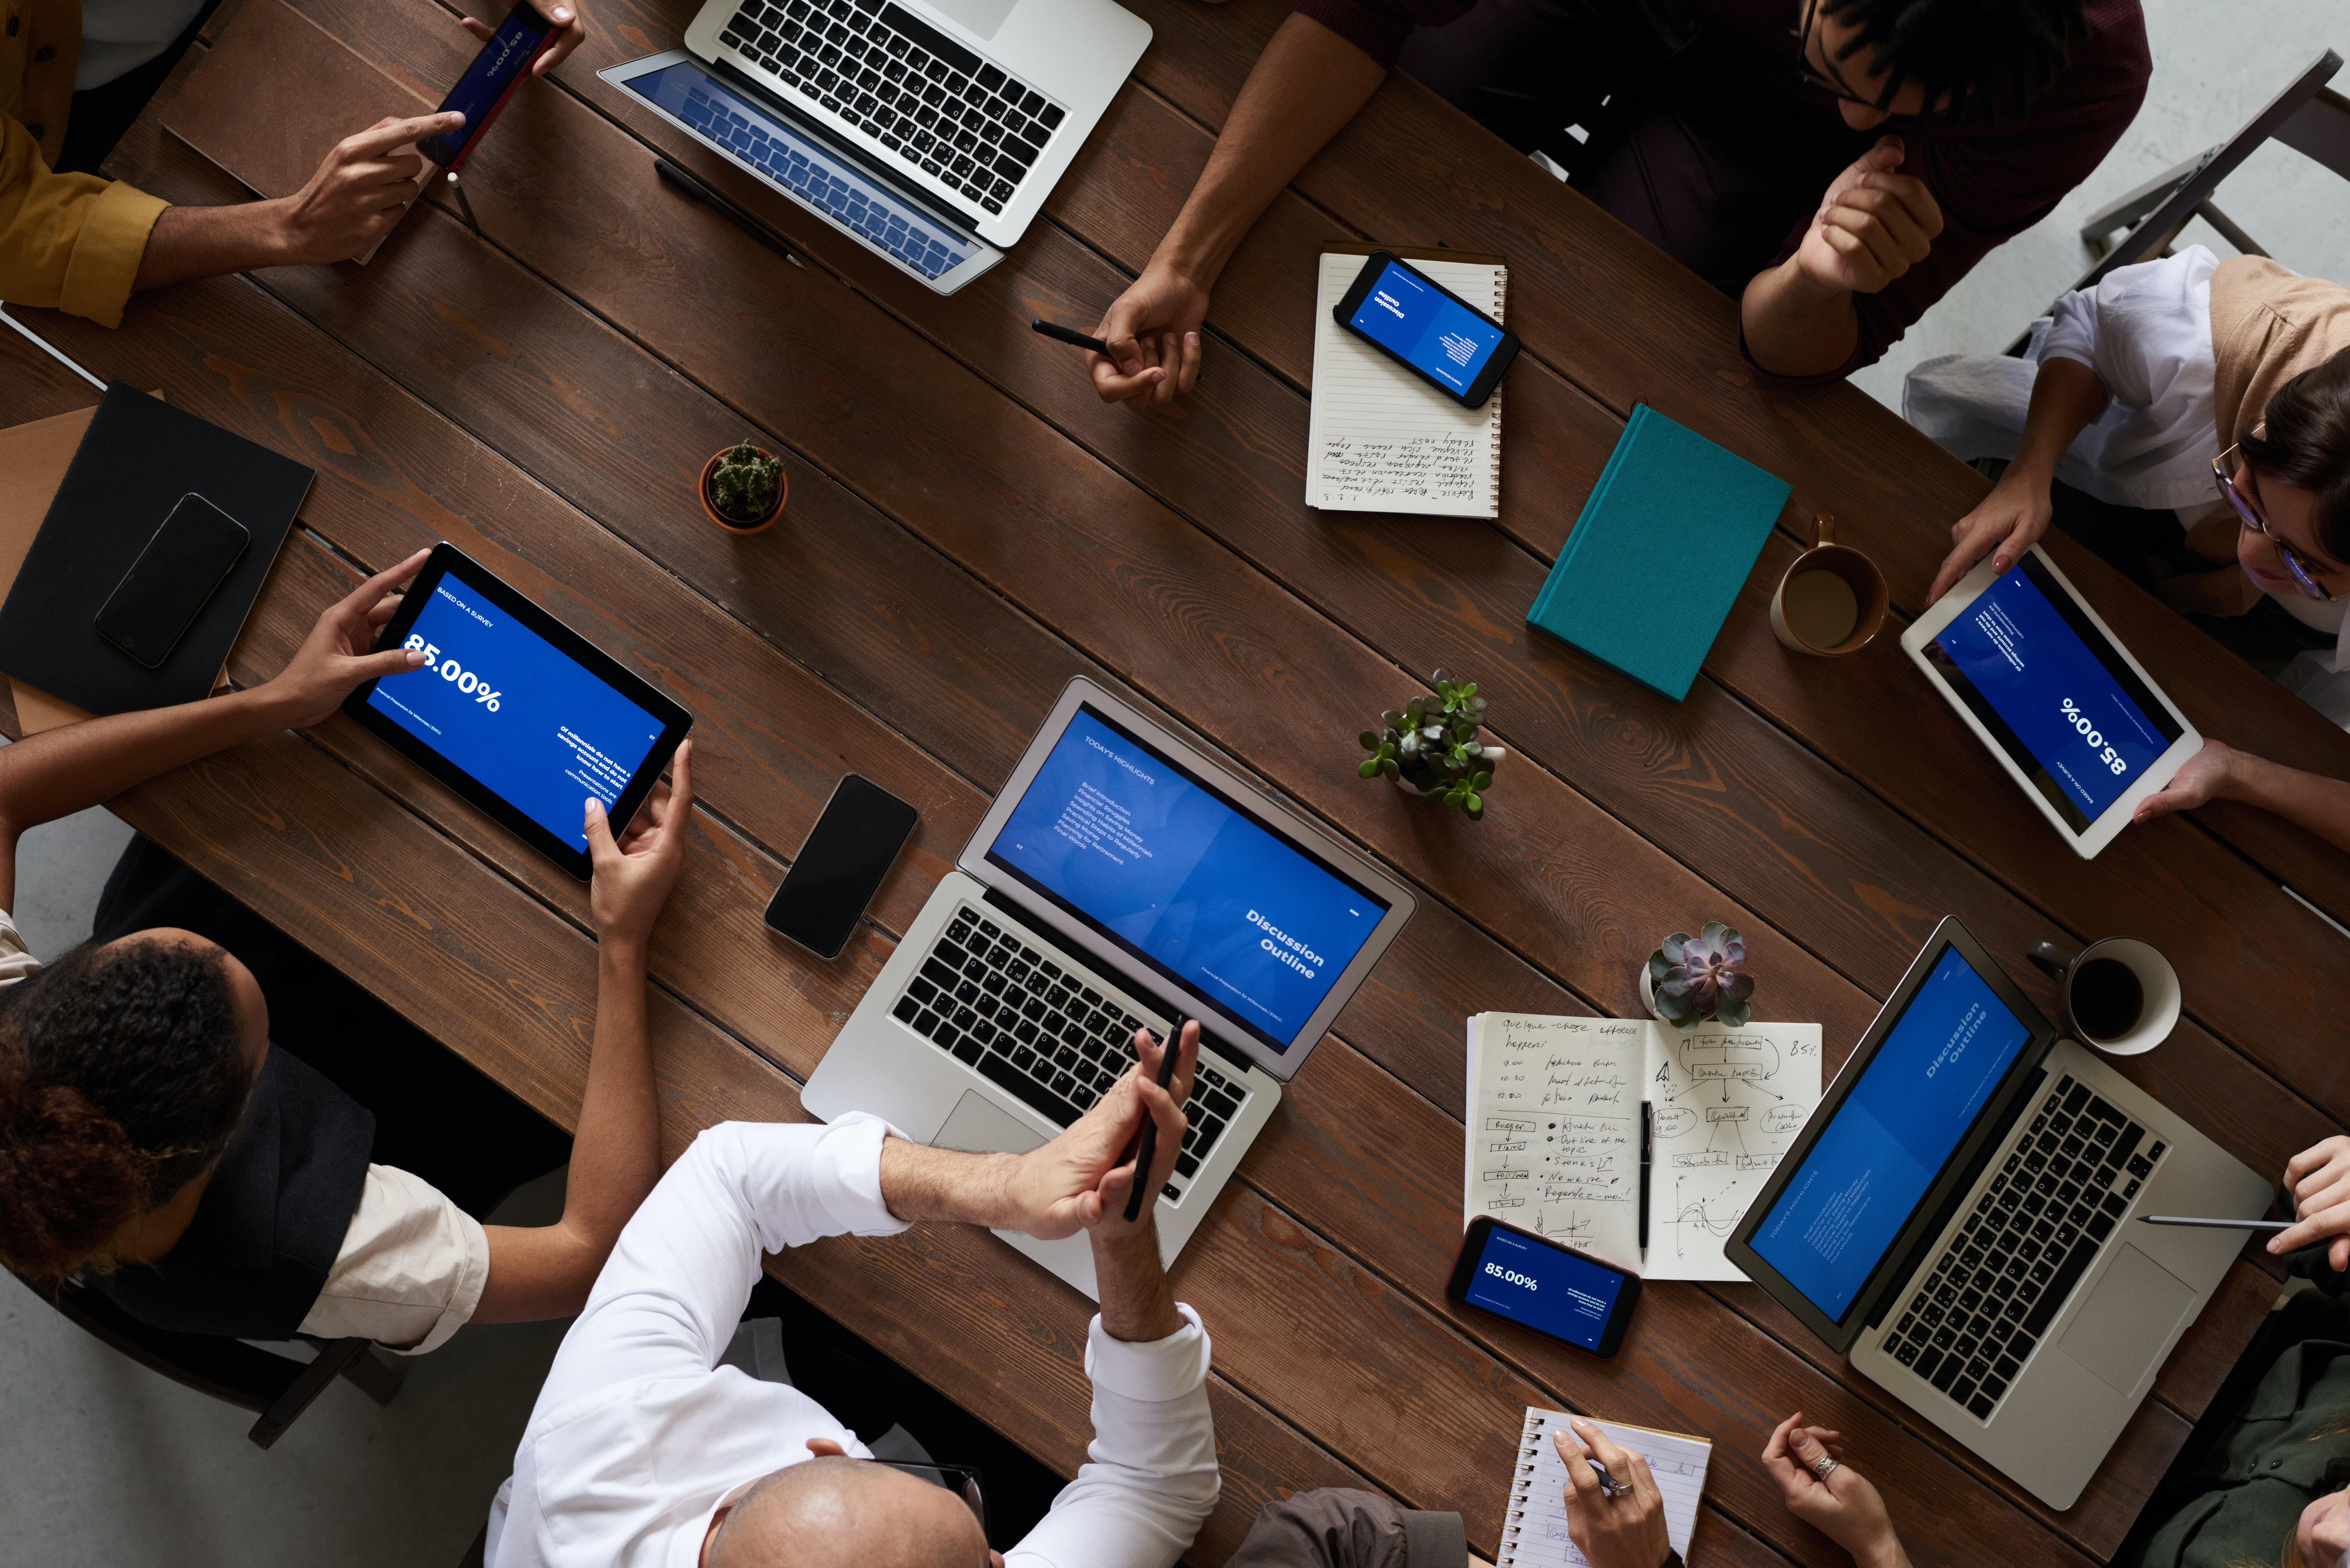
\includegraphics[height=0.3\textheight]{images/sociedad.jpg} \\
  			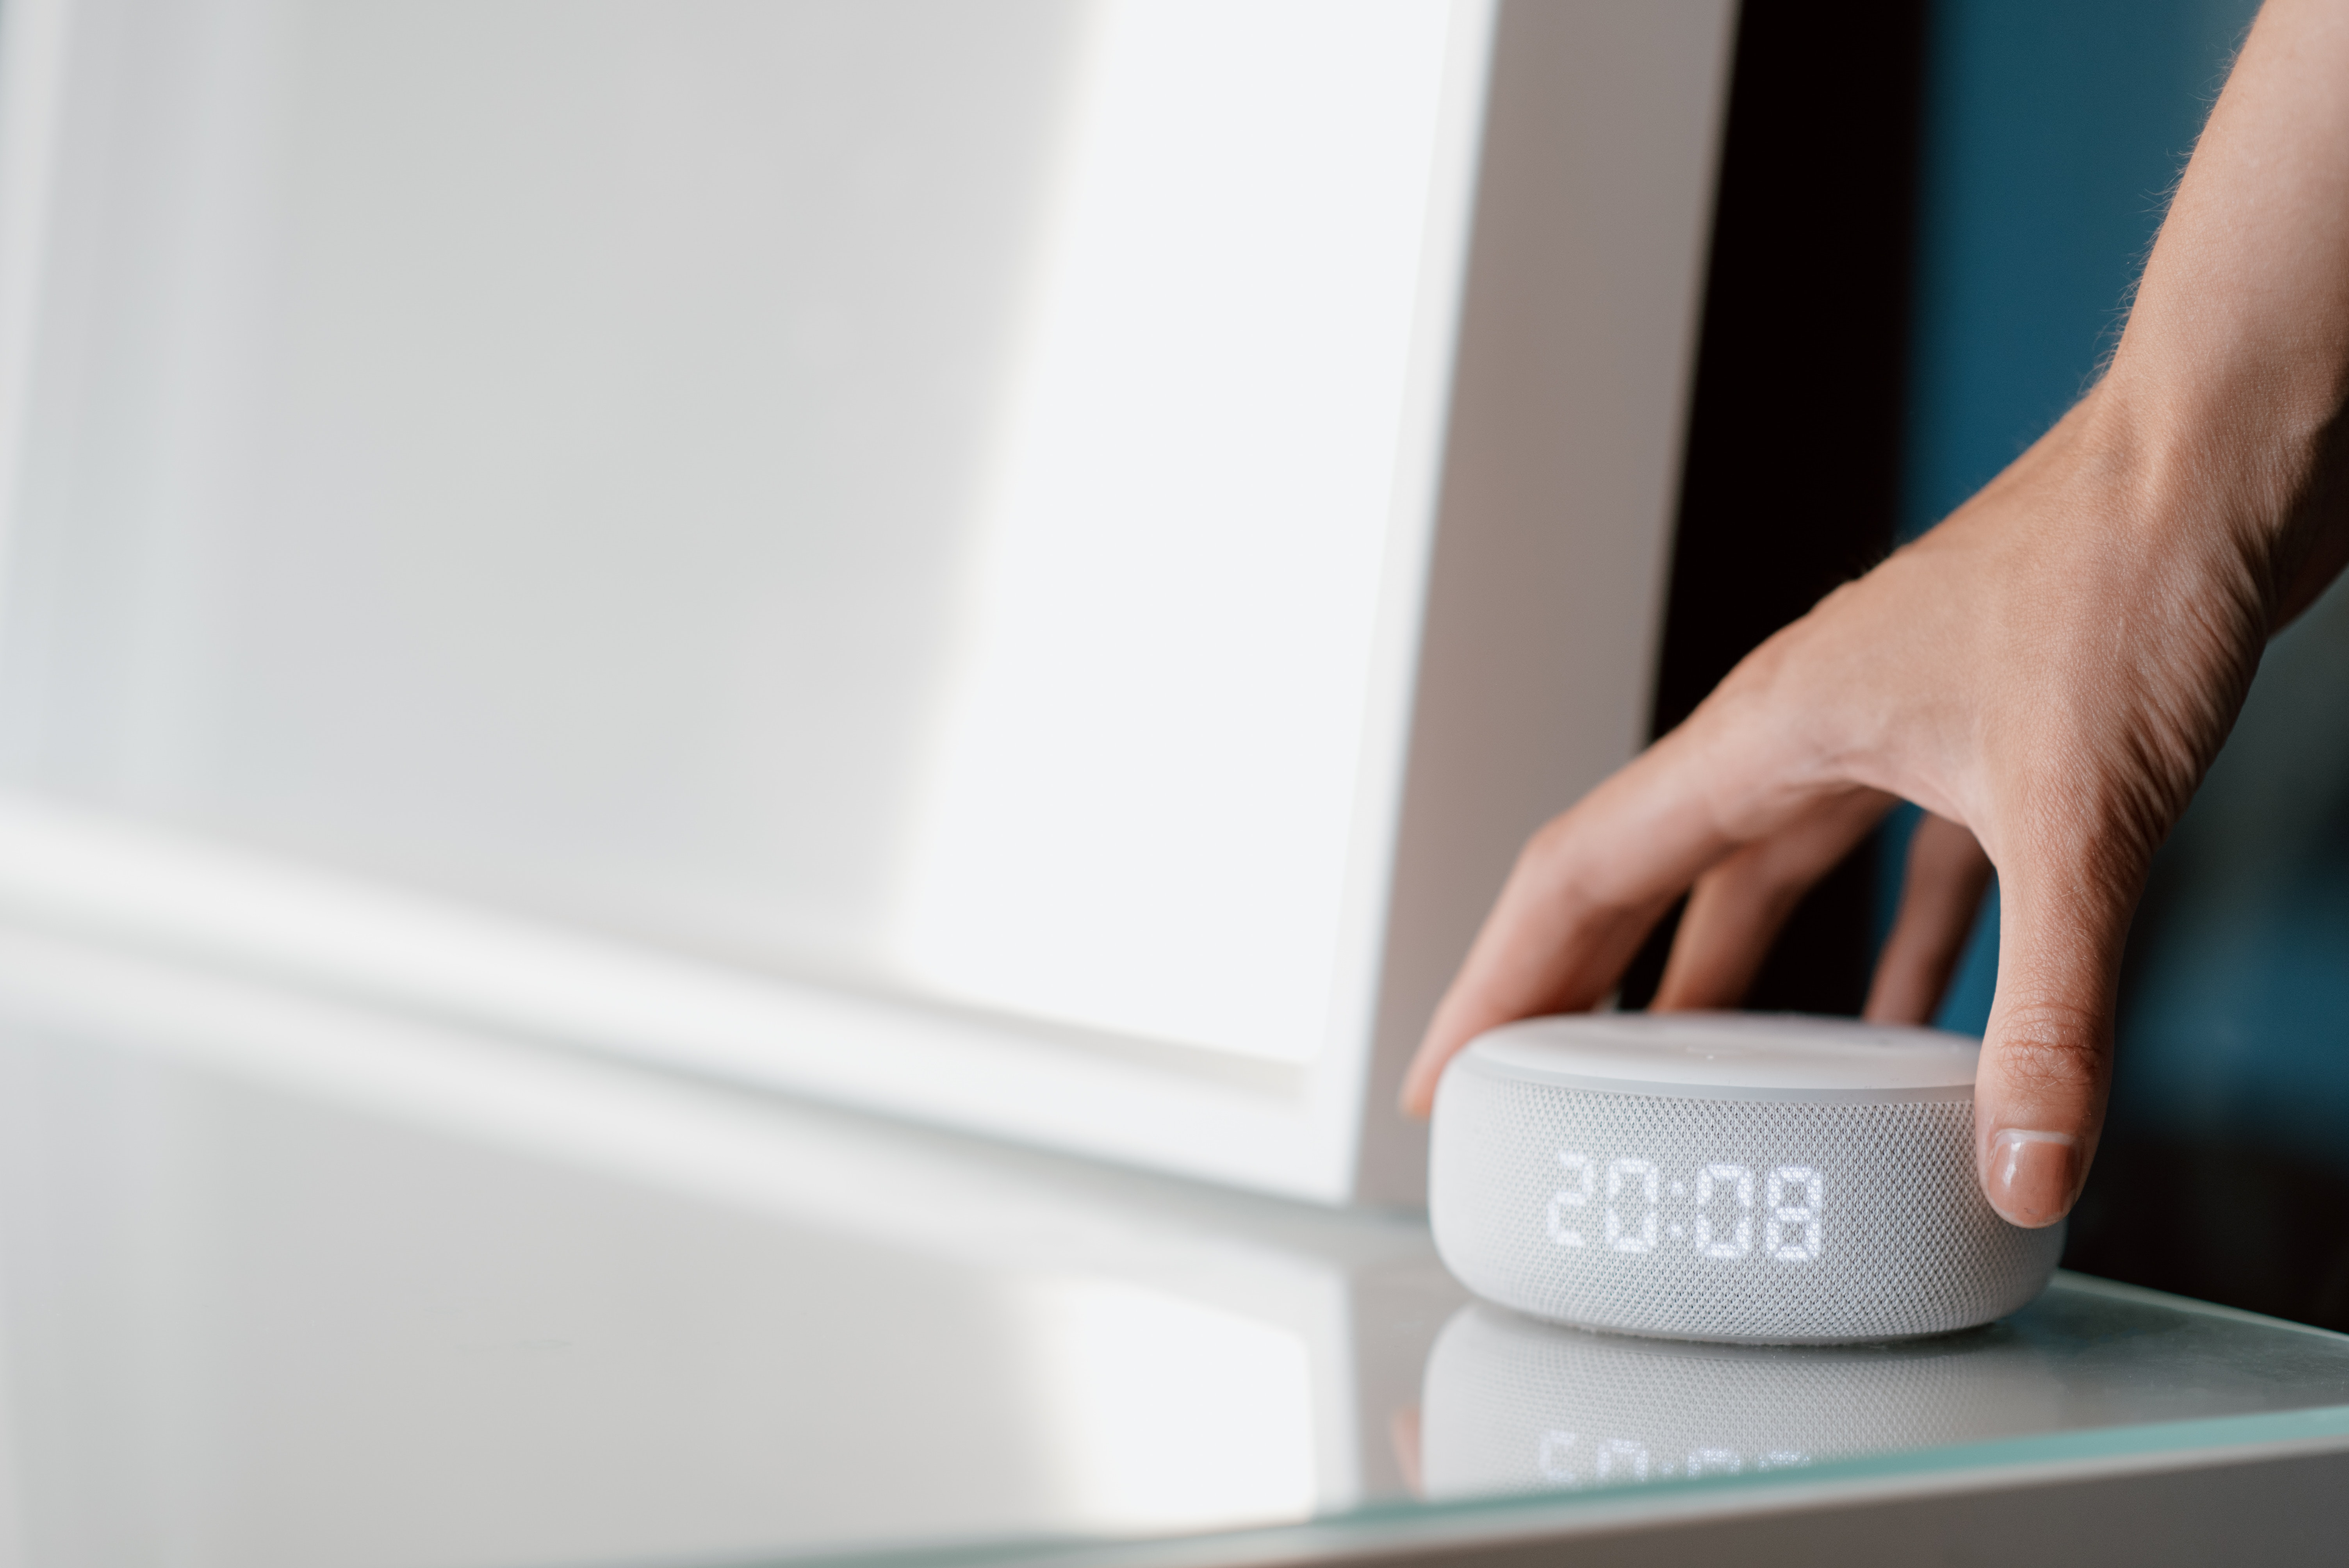
\includegraphics[height=0.3\textheight]{images/alexa.jpg}
  		\end{figure}
  	\end{minipage} \\
  	\end{tabular}
  \end{table}
\end{frame}

\begin{frame}{\insertsectionhead}
	\framesubtitle{Motivación > Desarrollo del Software y propiedad del código}
	\begin{table}[H]
		\begin{tabular}{lc}
			\begin{minipage}{0.45\textwidth}
				\begin{figure}[H]
					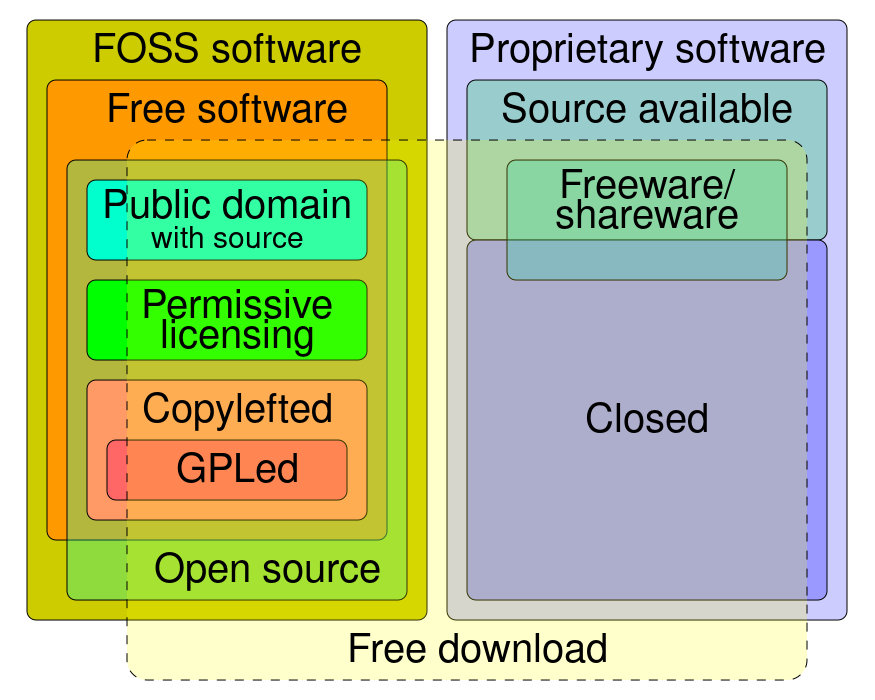
\includegraphics[width=\textwidth]{images/Software_Categories_expanded.png} \\
				\end{figure}
			\end{minipage}
		&
			\begin{minipage}{0.5\textwidth}
				\begin{itemize}
					\item  Necesidad de preparar soluciones que satisfagan las tareas más mecánicas y repetitivas. $\rightarrow$ Surgen empresas para desarrollar ese software.
					\item Ocultación y restricciones $\rightarrow$ ¿Por qué? ¿Hay alternativas?
					\item ¿En qué beneficia liberar el código? \cite{foss-marcojuridico}
					\item Licencias.
				\end{itemize}
			\end{minipage} \\
		\end{tabular}
	\end{table}
\end{frame}


%==============================================
\section{Estado del arte}
%==============================================

\subsection{}

\begin{frame}[fragile=singleslide]{\insertsectionhead}
  \framesubtitle{Una idea intuitiva de los Asistentes de Voz}
  \begin{figure}[H]
  	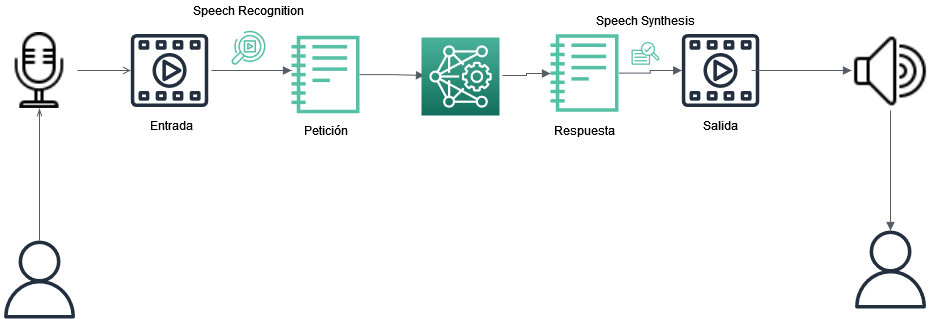
\includegraphics[width=\textwidth]{images/DiagramaIntuitivo.png}
  	\caption {Diagrama intuitivo del flujo de funcionamiento de un Asistente de Voz. \cite{sr-methods}}
  \end{figure}
  
\end{frame}

%==============================================
\section{El proyecto}
%==============================================

\begin{frame}
	\frametitle{\insertsectionhead}
	\framesubtitle{¿Qué se ha desarrollado?}
	\begin{itemize}
		\item Un Asistente de Voz.
		\item \textbf{Limitaciones}: Usar para el proyecto \underline{APIs libres}, en medida de lo posible.
		\item Programa resultante con licencia libre.
		
	\end{itemize}
\end{frame}



%==============================================
\section{Análisis}
%==============================================

\subsection{Comparando sistemas de SR > El experimento}
\begin{frame}{\insertsectionhead}
  \framesubtitle{\insertsubsectionhead}
  
  	\begin{figure}
  		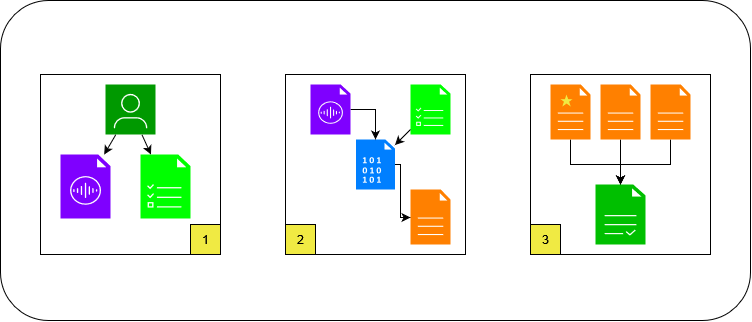
\includegraphics[height=0.45\textheight]{images/ProcesoExperimento.png}
  	\end{figure}
	
	\begin{alertblock}{Cálculo de WER y CER}
		\begin{center}
			$WER = \frac{I+S+R}{N}$
			\hspace{3cm}
			$CER = \frac{I_c+S_c+R_c}{N_c}$
		\end{center}
	\end{alertblock}
\end{frame}

%--------------------------------------
\subsection{Comparando sistemas de SR > Resultados}
\begin{frame}
  \frametitle{\insertsectionhead}
  \framesubtitle{\insertsubsectionhead}
  \begin{figure}
  	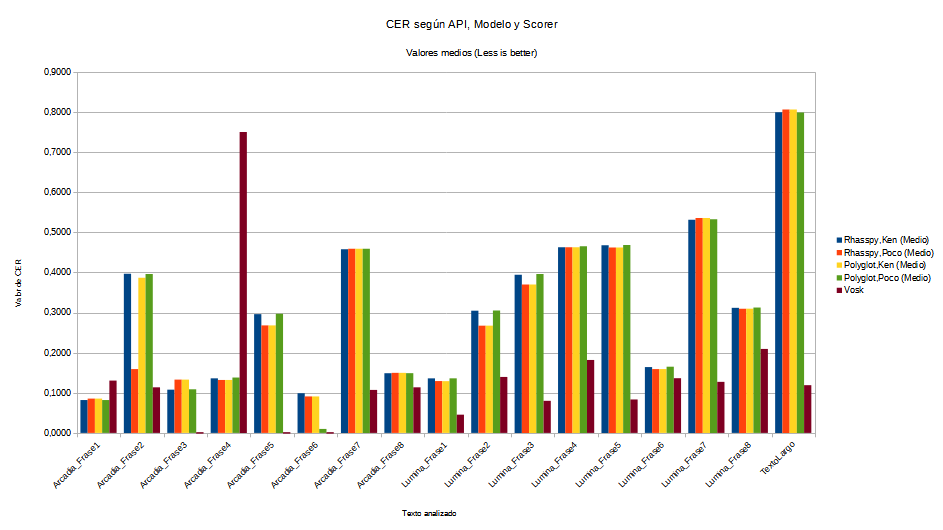
\includegraphics[width=0.45\textwidth]{images/CERMedios.png}
  	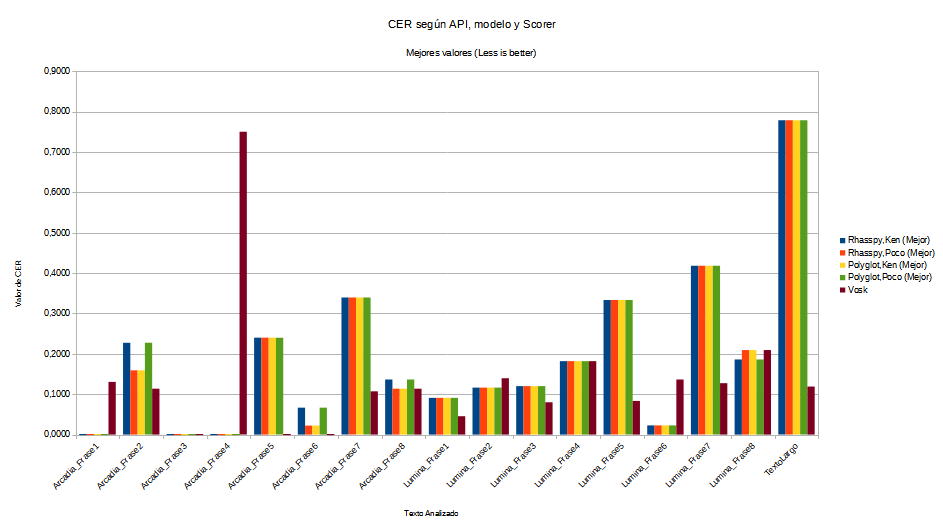
\includegraphics[width=0.45\textwidth]{images/CERMejores.png}
  	\caption{Valores medios y mejores del Ratio de Error de Caracteres}
  \end{figure}

\end{frame}

%--------------------------------------
\subsection{Comparando sistemas de SR > Resultados}
\begin{frame}
	\frametitle{\insertsectionhead}
	\framesubtitle{\insertsubsectionhead}
	\begin{figure}
		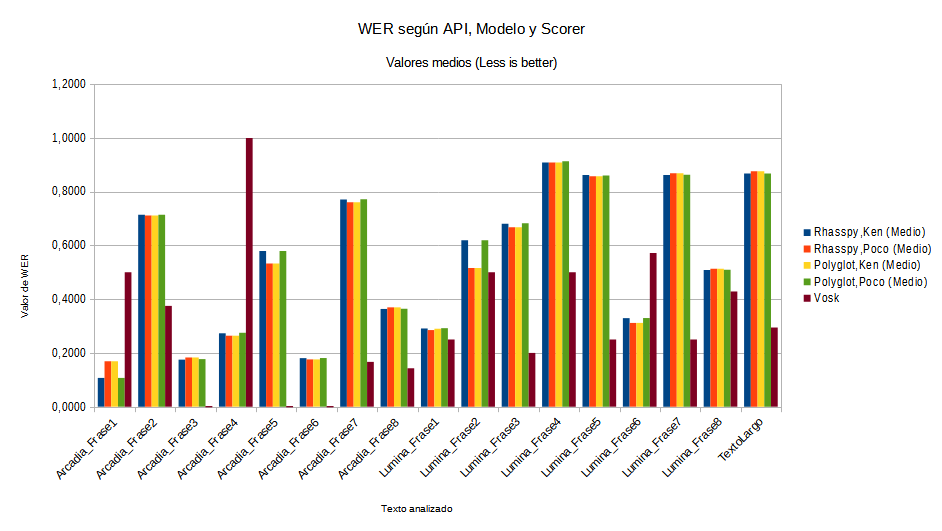
\includegraphics[width=0.45\textwidth]{images/WERMedios.png}
		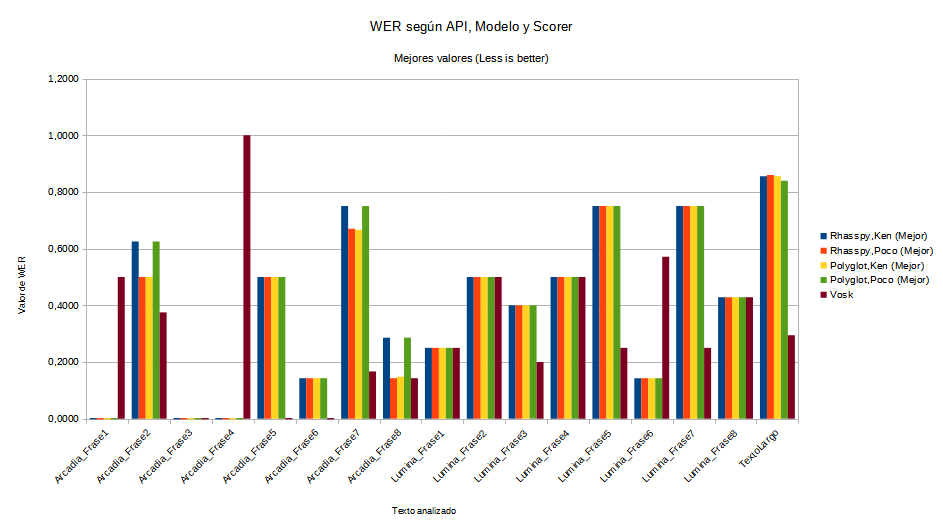
\includegraphics[width=0.45\textwidth]{images/WERMejores.png}
		\caption{Valores medios y mejores del Ratio de Error de Palabras}
	\end{figure}
	
\end{frame}



%--------------------------------------
\section{Diseño}
%--------------------------------------
\subsection{La arquitectura}
\begin{frame}
	\frametitle{\insertsectionhead}
	\framesubtitle{\insertsubsectionhead}
  \begin{figure}
  	\includegraphics[width=0.58\textwidth]{images/DiagramaArquitectónico.png}
  	\caption{Diagrama de la Arquitectura de Arcadia}
  \end{figure}
\end{frame}

%--------------------------------------
\subsection{Diagrama de clases}
\begin{frame}
	\frametitle{\insertsectionhead}
	\framesubtitle{\insertsubsectionhead}
	\begin{figure}
		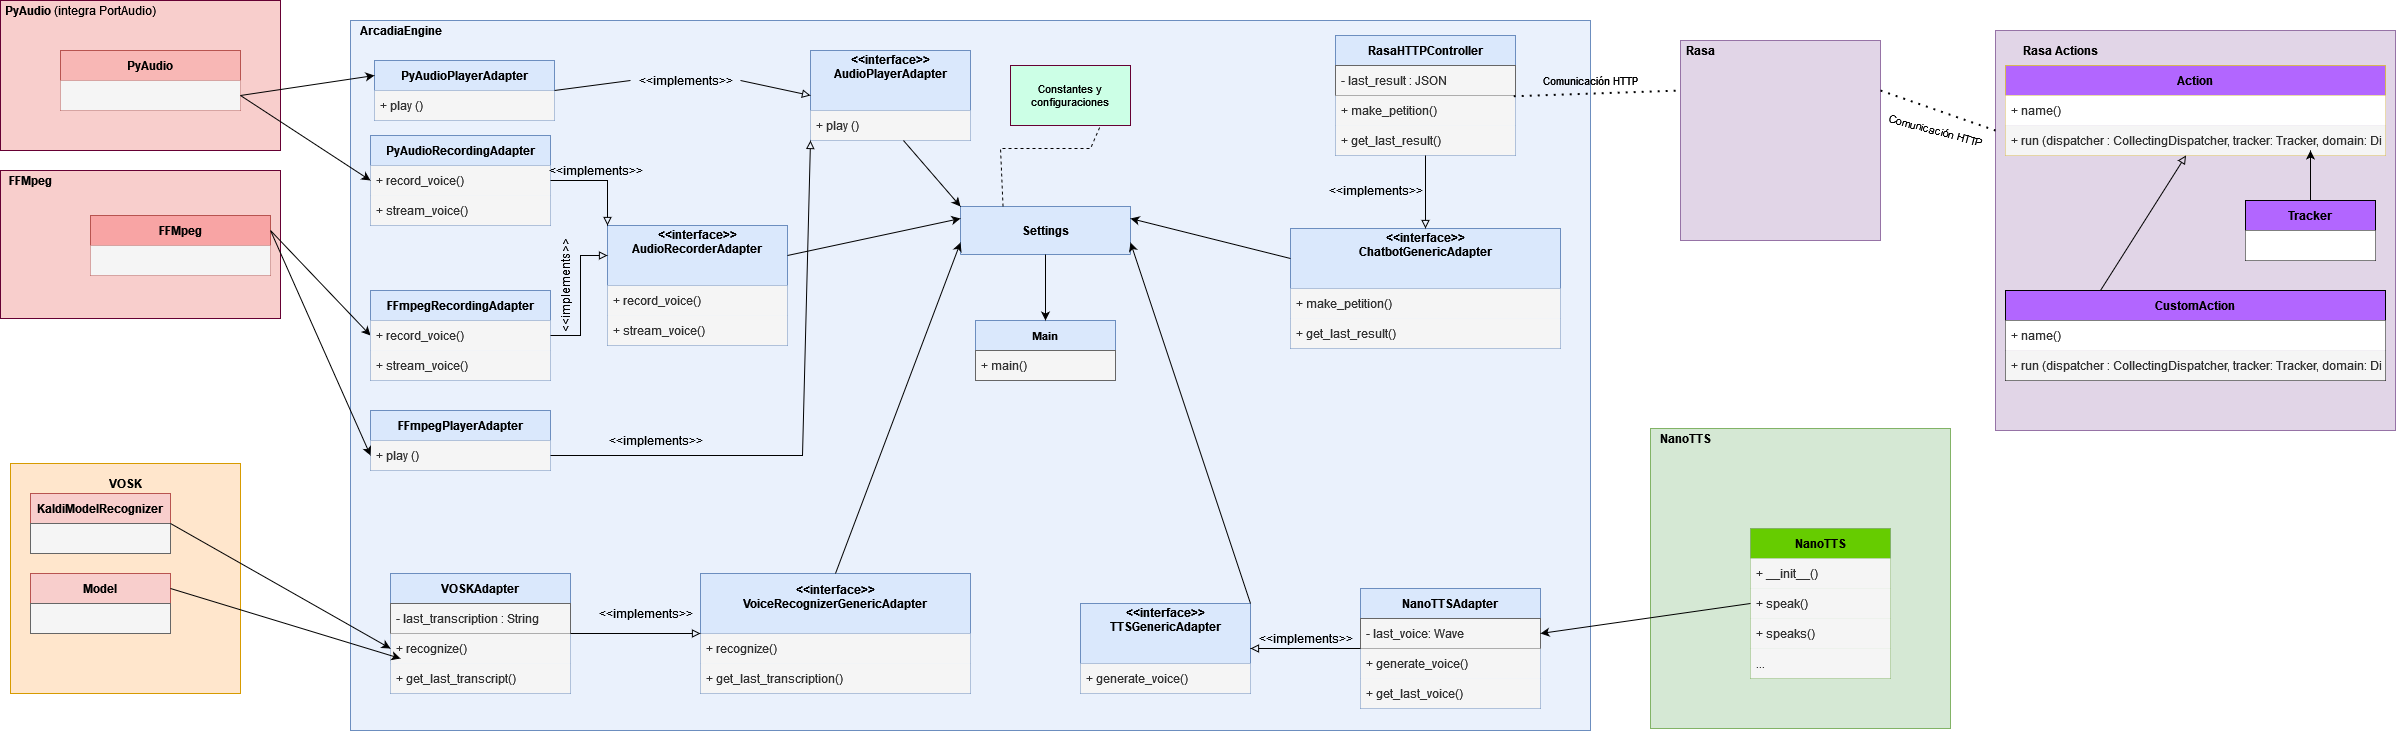
\includegraphics[width=\textwidth]{images/DiagramaClases_General.png}
		\caption{Diagrama de Clases de Arcadia}
	\end{figure}
\end{frame}

%==============================================
\section{Desarrollo}
%==============================================

\subsection{Sprints}
\begin{frame}
  \frametitle{\insertsectionhead}
  \framesubtitle{\insertsubsectionhead}
  \begin{table}[H]
  	\begin{tabular}{lc}
  		\begin{minipage}{0.4\textwidth}
  			\begin{enumerate}
  				\item Interacción Ordenador-Persona
  				\item Conectar preguntas y respuestas. Integración del flujo.
  				\item Funcionalidades y habilidades. \cite{rasa}
  				\item Documentación y cuidado del repositorio.
  			\end{enumerate}
  		\end{minipage}
  		& \begin{minipage}{0.55\textwidth}
  			\begin{figure}[H]
  				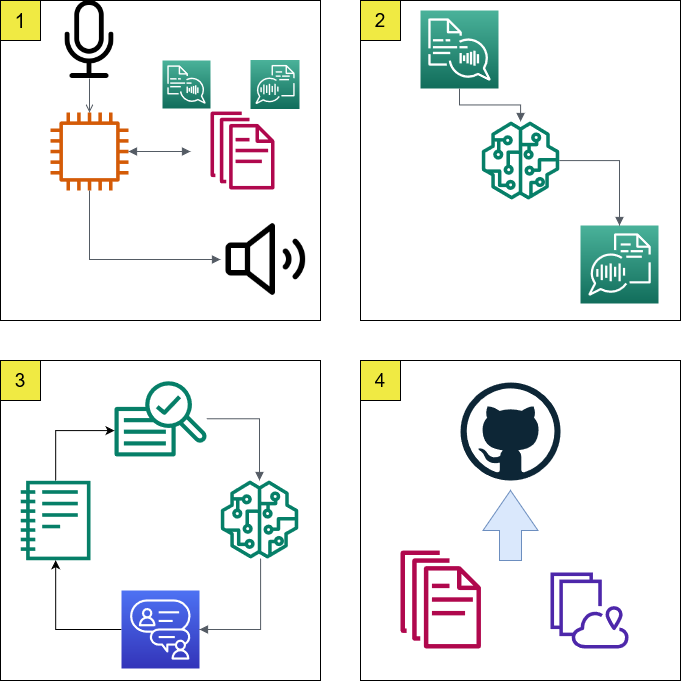
\includegraphics[width=0.7\textwidth]{images/Sprints.png} 
  			\end{figure}
  		\end{minipage} \\
  	\end{tabular}
  \end{table}
\end{frame}

%==============================================

\subsection{Tecnologías usadas}
\begin{frame}
	\frametitle{\insertsectionhead}
	\framesubtitle{\insertsubsectionhead}
	\begin{figure}
		
\includegraphics[width=0.65\textwidth]{images/TecnologiasUsadas.png}
	\end{figure}
\end{frame}


\subsection{Pruebas}
\begin{frame}
	\frametitle{\insertsectionhead}
	\framesubtitle{\insertsubsectionhead}
	\begin{table}[H]
		\centering
		\caption{Nº de pruebas de cada tipo según el sprint}
		\begin{tabular}{@{} lccc @{}}
			\toprule
			& \textbf{Sprint 1} & \textbf{Sprint 2}  & \textbf{Sprint 3} \\
			\midrule
			Pruebas unitarias  & 6 & 2 & - \\
			Pruebas de concepto/interacción  & 3  & 1 & - \\
			Pruebas beta  & - & - & 1 \\
			\bottomrule
		\end{tabular}
	\end{table}
\end{frame}


\subsection{Demo Técnica}
\begin{frame}
	\frametitle{\insertsectionhead}
	\framesubtitle{\insertsubsectionhead}
	\begin{figure}[H]
		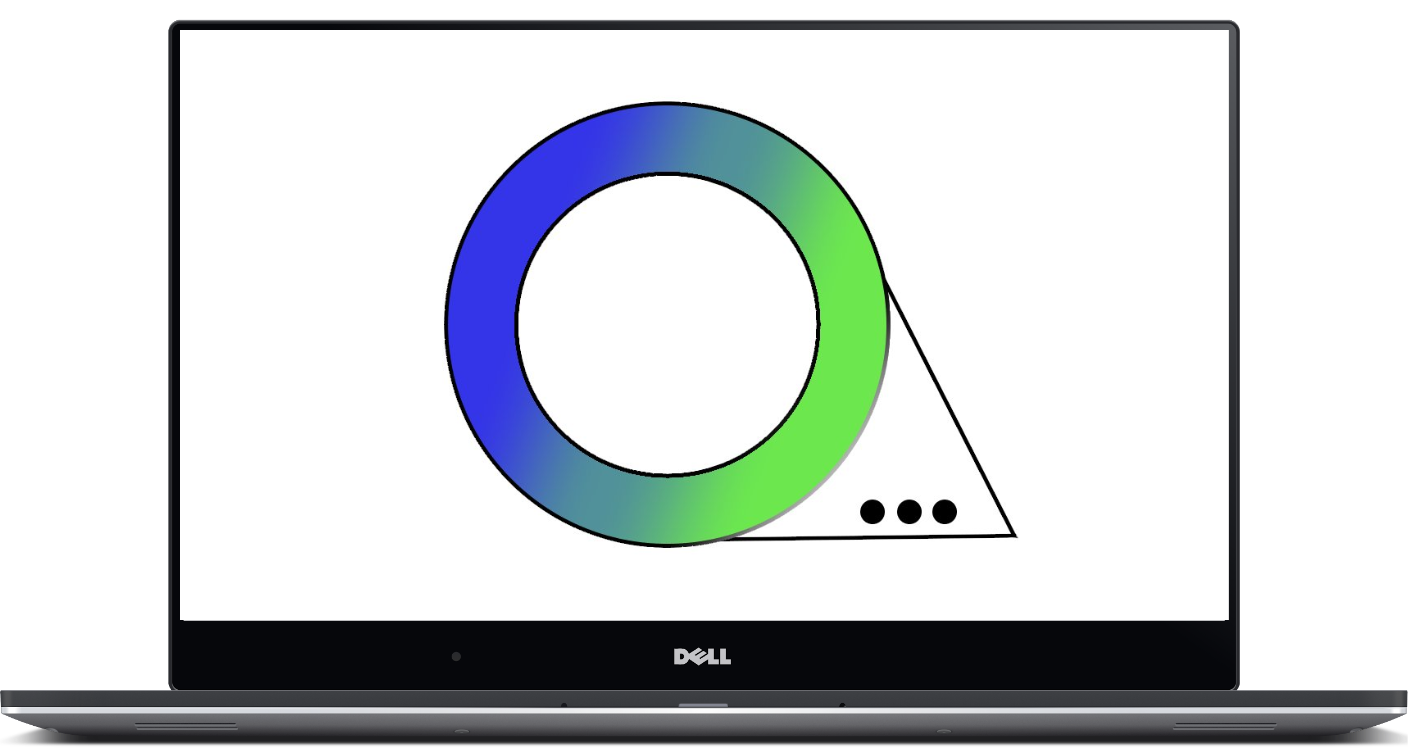
\includegraphics[width=0.6\textwidth]{images/Demo.png}
	\end{figure}
\end{frame}

%==============================================

%==============================================
\section{Conclusiones}
%==============================================

\begin{frame}
	\frametitle{\insertsectionhead}
	
	\begin{itemize}
		\item Análisis etnográfico de:
		\begin{itemize}
			\item Asistentes de Voz
			\item Software Libre / Open Source
		\end{itemize}
		\item Creación de aplicación:
		\begin{itemize}
			\item Asistente de Voz
			\item Limitado a APIs Libres/Abiertas
			\item Facilidad de uso
			\item Código visible a cualquiera $\rightarrow$ Disponible en GitHub
		\end{itemize}
		\item Difusión del conocimiento.
	\end{itemize}
	
\end{frame}

\begin{frame}[allowframebreaks]{Bibliografía}

  \bibliography{demo}
  \bibliographystyle{abbrv}

\end{frame}

\begin{frame}{}
	
	\Huge{¡Muchas gracias por su atención!}
	
	\normalsize{¿Dudas, preguntas, cuestiones...?}
\end{frame}
